\section{Auswertung}
\label{sec:Auswertung}

\subsection{Geometrische Daten der Messapperatur}
Im weiteren werden der Kugelradius $R_\text{K}$, die Kugelmasse $m_\text{K}$, das Trägheitsmoment der Kugelhalterung $\theta_\text{H}$, die Windungszahl der Helmholzspule $N$ und der Radius der Helmholzspule $R_\text{H}$ aufgelistet.
\begin{align*}
  R_\text{K} &= (\num{0.02538 +- 0.00001}) \ \text{m} \\
  m_\text{K} &= (\num{0.5122 +- 0.0002}) \ \text{kg} \\
  \theta_\text{H} &= 2.25 \cdot 10^{-6} \ \text{kg m}^2 \\
  N &= 390 \\
  R_\text{H} &= 0.078 \ \text{m}
\end{align*}
Die Abmessungen des Drahtes sind in der folgenden Tabelle aufgeführt.

\begin{table}[H] %Abmessungdes Drahtes
  \centering
  \begin{tabular}{c | c | c}
    \toprule
    & L / m & 2R / $10^{-3}$ \ m \\
    \midrule
    & 0.598 & 0.210 \\
    & 0.597 & 0.205 \\
    & 0.600 & 0.210 \\
    &       & 0.200 \\
    &       & 0.205 \\
    \bottomrule
    Mittelwert(nach Gl. (\ref{eqn:ave}))         & 0.5983 & 0.2060 \\
    Standardabweichung(nach Gl. (\ref{eqn:std})) & 0.0008 & 0.0004 \\
    \bottomrule
  \end{tabular}
  \caption{Die Abmessung des Drahtes.}
  \label{tab:Messwerte}
\end{table}

Das Gesamtträgheitsmoment ergibt sich aus der Summation von dem Trägheitsmoment der Kugel(siehe Gl. (\ref{eqn:theta})) und der Halterung.
\begin{align*}
  \theta_\text{k} & = (\num{1.3197 +- 0.0012}) \cdot 10^{-4} \ \text{kg m}^2 \\
  \theta_\text{ges} & = \theta_\text{K} + \theta_\text{H} = (\num{1.3422 +- 0.0012}) \cdot 10^{-4} \ \text{kg m}^2
\end{align*}

\subsection{Bestimmung des Schubmoduls G und der anderen elastischen Konstanten}
Mit den Tabellen \ref{tab:Messwerte} und \ref{tab:Periodendauer1} und der Gleichung (\ref{eqn:G}) folgt der Schubmodul $G$ zu
\begin{align*}
  G = (\num{4.99 +- 0.04}) \cdot 10^{10} \frac{\text{N}}{\text{m}^2} \ .
\end{align*}

\begin{table}[H] %Periodendauer ohne Magnet
  \centering
  \begin{tabular}{c c}
    \toprule
    & T / s \\
    \midrule
    1. & 18.798 \\
    2. & 18.800 \\
    3. & 18.800 \\
    4. & 18.751 \\
    5. & 18.794 \\
    6. & 18.799 \\
    7. & 18.798 \\
    8. & 18.795 \\
    9. & 18.797 \\
    10.& 18.800 \\
    \bottomrule
    Mittelwert(nach Gl. (\ref{eqn:ave})) & 18.793 \\
    Standardabweichung(nach Gl. (\ref{eqn:std})) & 0.014 \\
    \bottomrule
  \end{tabular}
  \caption{Periodendauer der Schwingung ohne Magnet.}
  \label{tab:Periodendauer1}
\end{table}

Die Werte für den Elastizitätsmodul und den Schubmodul wurden vorgegeben:
\begin{align*}
  E = 21 \cdot 10^{10} \frac{\text{N}}{\text{m}^2}
\end{align*}
\begin{align*}
  G = 8.2 \cdot 10^{10} \frac{\text{N}}{\text{m}^2}
\end{align*}
Im weiteren Verlauf wird das gegebene $G$ verwendet. Mit Hilfe von $E$ und $G$ werden nun die poissonsche Querkontraktionszahl $\mu$ und der Kompressionsmodul $Q$ bestimmt. Mit den Gleichungen (\ref{eqn:pois}) und (\ref{eqn:komp}) ergeben sich:
\begin{equation}
  \mu = \frac{E}{2G} - 1 = 0.28
\end{equation}
und
\begin{equation}
  Q = \frac{E}{-6 \mu + 3} = 1.59 \cdot 10^{11} \frac{\text{N}}{\text{m}^2} \ .
\end{equation}

\subsection{Bestimmung des magnetischen Momentes $m$}
Zur Bestimmung des magnetischen Momentes, wird die Periodendauer $T_\text{m}$ in Abhängigkeit vom Spulenstrom $I$ gemessen, sämtliche Messwerte sind in Tabelle \ref{tab:Periodendauer3} angegeben.

\begin{table}[H] %Schwingungsdauern in Abhängigkeit vom Spulenstrom
  \centering
  \begin{tabular}{c | c | c | c | c | c}
    & I = 0.2A & I = 0.4A & I = 0.6A & I = 0.8A & I = 1.0A \\
    \midrule
    $T_\text{m}$ / s & 17.184 & 16.027 & 15.081 & 14.152 & 13.197 \\
    $T_\text{m}$ / s & 17.166 & 15.992 & 15.048 & 14.104 & 13.251 \\
    $T_\text{m}$ / s & 17.378 & 16.005 & 15.052 & 14.142 & 13.163 \\
    $T_\text{m}$ / s & 17.333 & 16.006 & 15.041 & 14.109 & 13.244 \\
    $T_\text{m}$ / s & 17.336 & 15.992 & 15.026 & 14.104 & 13.174 \\
    \bottomrule
    Mittelwert(nach Gl. (\ref{eqn:ave})) & 17.280 & 16.004 & 15.050 & 14.122 & 13.210 \\
    Standardabweichung(nach Gl. (\ref{eqn:std})) & 0.090 & 0.013 & 0.018 & 0.021 & 0.040 \\
    \bottomrule
  \end{tabular}
  \caption{Messwerte für die Schwingungsdauern in Abhängigkeit vom Spulenstrom.}
  \label{tab:Periodendauer3}
\end{table}

Zunächst wird über den Spulenstrom das Magnetfeld im Zentrum der Spule mit Hilfe von Gleichung (\ref{eqn:B}) berechnet.
\begin{equation}
  B = \frac{8 \mu_0 N I}{\sqrt{125}R} \ .
  \label{eqn:B}
\end{equation}
Mit $\mu_0 = 4 \pi \cdot 10^{-7} \ \frac{\text{N}}{\text{A}^2}$.
Nun kann Gleichung (\ref{eqn:Tmag}) zu
\begin{equation}
  mB + D = \frac{4 \pi^2 \theta}{T_\text{m}^2}
  \label{eqn:MagMoment}
\end{equation}
umgestellt werden. Das magnetische Moment wird nun mit Hilfe einer linearen Regression bestimmt. Die Steigung der Geraden entspricht dann dem magnetischen Moment. In Tabelle \ref{tab:BUndMehr} sind $B$ und $\frac{4 \pi^2 \theta}{T_\text{m}^2}$ aufgelistet.

\begin{table}[H]
  \centering
  \begin{tabular}{c c}
    \toprule
    B / mT & $\frac{4 \pi^2 \theta}{T_\text{m}^2}$ / $10^{-4}$ \ Nm \\
    \midrule
    0.68 & 1.77 \\
    1.36 & 2.07 \\
    2.04 & 2.34 \\
    2.72 & 2.66 \\
    3.40 & 3.04 \\
    \bottomrule
  \end{tabular}
  \caption{}
  \label{tab:BUndMehr}
\end{table}

In Abbildung \ref{fig:magMoment} ist $B$ gegen $\frac{4 \pi^2 \theta}{T_\text{m}^2}$ aufgetragen und es wurde zusätzlich eine Ausgleichgerade eingezeichnet.

\begin{figure}[H]
  \centering
  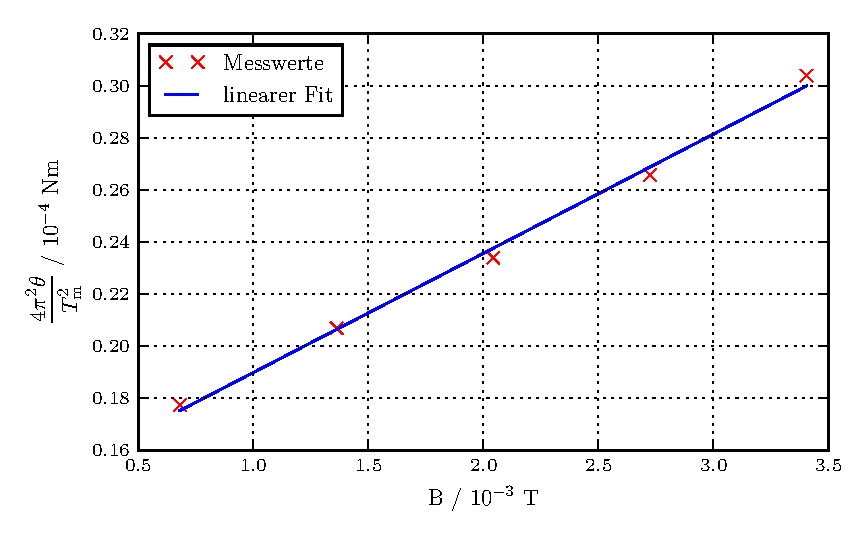
\includegraphics[height=7cm]{MagnetischesMoment.pdf}
  \caption{Messpunkte und Ausgleichsgerade zur Messung des magnetischen Moments $m$.}
  \label{fig:magMoment}
\end{figure}

Damit folgt das magnetische Moment $m$ zu
\begin{equation}
  m = (\num{4.58 +- 0.18}) \cdot 10^{-3} \frac{\text{Nm}}{\text{T}}
\end{equation}


\subsection{Bestimmung der Horizontalkomponente des Erdmagnetfeldes}
Aufgrund der Horizontalkomponente des Erdmagnetfeldes, wirkt auf den Magneten in der Kugel ein zusätzliches Drehmoment. Dazu muss der Dipolmagnet in der Kugel in Richtung des Erdmagnetfeldes zeigen. Je nach Orientierung geht davon eine Vergrößerung oder Verkleinerung der Periodendauer aus. Für die Periodendauer im Erdmagnetfeld siehe Tabelle \ref{tab:Periodendauer2}.

\begin{table}[H] %Periodendauer mit Magnet
  \centering
  \begin{tabular}{c c}
    \toprule
    & $T_\text{E}$ / s \\
    \midrule
    1. & 18.638 \\
    2. & 18.607 \\
    3. & 18.582 \\
    4. & 18.592 \\
    5. & 18.625 \\
    6. & 18.629 \\
    7. & 18.613 \\
    8. & 18.588 \\
    9. & 18.599 \\
    10.& 18.620 \\
    \bottomrule
    Mittelwert(nach Gl. (\ref{eqn:ave})) & 18.609 \\
    Standardabweichung(nach Gl. (\ref{eqn:std})) & 0.018 \\
    \bottomrule
  \end{tabular}
  \caption{Periodendauer der Schwingung mit Magnet.}
  \label{tab:Periodendauer2}
\end{table}

Die Horizontalkomponente lässt sich aus Gleichung (\ref{eqn:MagMoment}) nach $B$ umgestellt bestimmen.
\begin{equation}
  B_\text{h} = \frac{4 \pi^2 I_\text{ges}}{m} \left(\frac{1}{T_\text{E}^2} - \frac{1}{T^2} \right) = (\num{65.0 +- 8.0}) \ \text{µT}
\end{equation}
